Several regression models for manifold-valued data have been proposed, a majority of 
which are nonparametric \citep{jayasumanakernel,banerjee2015nonlinear}. 
%             , and make use of various distance metrics.
Because of the longitudinal nature of our dataset (and recruitment considerations in neuroimaging studies),
%it is not common for  
sample sizes do not exceed a few hundred participants (typically much smaller). 
%Since in longitudinal neuroimaging study, the number of subjects and the number of their visits is limited. 
We have found that generally, in this regime, parametric methods are better suited and also offer other benefits for downstream applications. 
%Our description below will, therefore, 
Next, we will give a simple parametric model for this problem. 
\begin{figure*}[t]
  \centering
  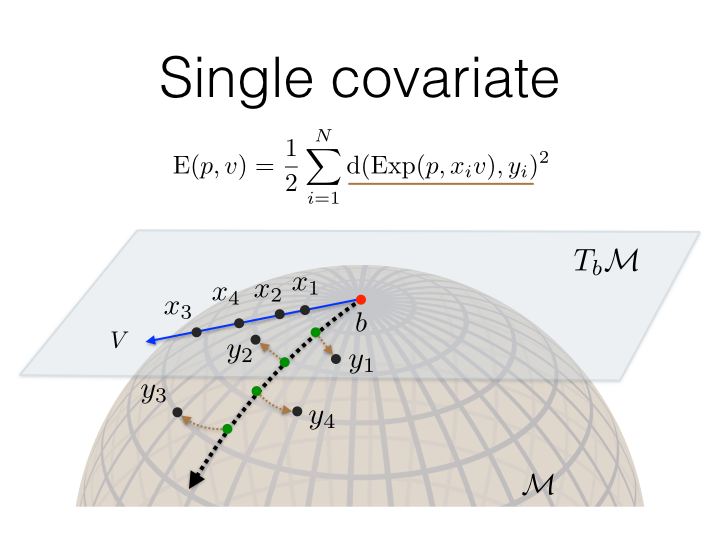
\includegraphics[width=0.49\textwidth,trim={10 40 10 220},clip]{3_covtraj/figs/MGLM1.png}
  %
    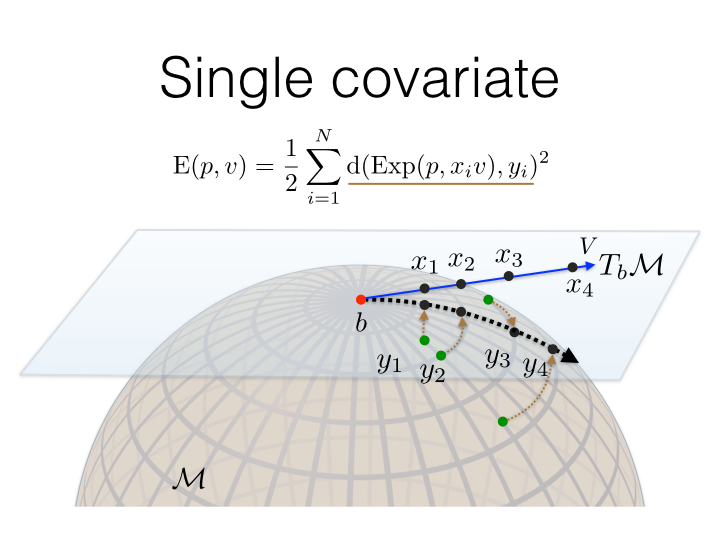
\includegraphics[width=0.49\textwidth,trim={10 40 10 220},clip]{3_covtraj/figs/MGLM2.png}
  \caption[Group-wise comparisons of manifold trajectories]{\label{fig:manifold}Group-wise MMGLM: The left and right figures represent two linear models on the $\SPD(p)$ manifold. Points $x_i$ in the tangent space are our covariate or predictor, and points $y_i$ in the manifold space represent $\SPD(p)$ matrices. In our regression setting, we wish to minimize the error (brown curves) between the estimation and the sample points. Because each linear model has a different base point, the trajectories cannot be directly compared as in the Euclidean setting.}
\end{figure*}
Let $x$ and $y$ be vectors in $\RR^p$ and $\RR^{p'}$ respectively.
\begin{definition} (Standard GLM.) The Euclidean multivariate multilinear model is 
{\begin{equation}
	\begin{split}
	y  = \beta^0 + \beta^{1} x^{1} + \beta^{2} x^{2} + \ldots +\beta^{p} x^{p} + \epsilon
	\end{split}
	\label{eq:generallinear}
	\end{equation}}
where $\beta^0$, $\beta^{i}$ and the error $\epsilon$ are in $\RR^{p}$ and $x = [x^1 \ldots x^p ]^{T}$ are the 
predictor variables.
\end{definition}
Henceforth, we will use the terms \textit{covariate} and \textit{predictor} interchangeably to describe those specific features we wish to control for in our model (e.g., time-points in our experiments).
For manifold-valued data, we adapt the formulation proposed by \cite{hjkimcvpr2014}.
\begin{definition} The Manifold Multivariate General Linear Model (MMGLM) is defined as 
{\begin{equation}
	\begin{split}
	&\min_{b \in \Mc, \forall j, V^j \in T_{b}\Mc} \quad \frac{1}{2} %\sum_{i=1}^{N}d(\EXP(p, {\sum_{j=1}^{n}v^j x_{i}^{j}}),y_i)^2,
	\sum_{i=1}^{N}d(\EXP(b, \textbf{V} x_i),y_i)^2,
	\end{split}
	\label{eq:multigr}
	\end{equation}}
where $\BV x_i \defeq \sum_{j=1}^{n}V^j x_{i}^{j}$, and $d(\cdot, \cdot)$ is the geodesic distance between $\hat{y}_i:=\EXP(b, \textbf{V} x_i)$ and $y_i$. 
\end{definition}
This formulation generalizes \eqref{eq:generallinear}, by replacing the intercept $\beta^0$ and each vector $\beta^j$ for a covariate with a 
base point $b \in \Mc$ and a geodesic basis $V^j \in T_{b}\Mc$ respectively. The geodesic basis $V^j$ at $b$ parameterizes a geodesic curve $\EXP(b,V^jx^j)$.
%for a manifold-valued \textit{dependent} variable is,
%It is clear that in MMGLM each covariate parameterizes a geodesic curve $\EXP(p, v^j x_i^j)$ on $\Mc$. 
Intuitively, this model is a ``generalized'' linear model with the inverse exponential map $\EXP^{-1}$ (or logarithm map $\LOG$) as a 
`link' function \citep{hjkimcvpr2014,cornea2016regression}. When the covariate/predictors are univariate, we will obtain a single geodesic curve, modeled via 
the so-called Geodesic Regression \citep{fletcher2013geodesic}.

\subsection{Efficient Estimation of Trajectories}
\label{sec:effest}
The objective in \eqref{eq:multigr}, can be solved by both gradient descent \citep{fletcher2013geodesic,hjkimcvpr2014} and MCMC methods \citep{cornea2016regression}. 
Unfortunately, these schemes can be expensive, especially when the dimension of the manifold is large. Further, if the algorithm needs to be run a 
large number of times, the computational footprint quickly becomes prohibitive. 
Motivated by these considerations, we use a so-called log-Euclidean approximate algorithm introduced in \cite{hjkimcvpr2014} with some adaptations, which requires mild assumptions on the manifold-valued data. 

Recall that in classical ordinary least squares (OLS), 
the regression curve goes through the mean of covariates and response variables, i.e., $y-\bar{y} = \beta(x-\bar{x})$.
Similarly, we assume that geodesic curves go through the mean of response variables on the manifold. Then, the base point, or intercept, ``$b$'' in \eqref{eq:multigr} can be approximated by the {\em manifold-valued mean of the sample points}, the Karcher mean \citep{karcher1977riemannian}. The propositions derived from \cite{hjkimcvpr2014} lead directly to the following. 
\begin{proposition}
Let $\bar{C}$ be the unique Karcher mean of a sufficiently close set of covariance matrices that lie on a curve $\Omega$. Then $\bar{C} \in \Omega$, and for some tangent vector $V \in T_{\bar{C}}\Mc$ and each $C$, there exists $x \in \mathbb{R}$ such that $C = \EXP(\bar{C},Vx)$. 	
\end{proposition}
This allows us to bypass the fairly involved variational procedure to estimate the base point $b$.

With this approximation of $\hat{b}$ via $\bar{y}$, the remaining variables to optimize are the tangent vectors $\BV$. 
We do so by taking advantage of log-Euclidean schemes. Once the base point is established as the Karcher mean, each data point on the manifold is projected into the tangent space at that point: $\LOG(\bar{y},y)$. These ``centered" points $\tilde{y}$ are now Euclidean, and if the covariates are centered as well ($\tilde{x}$), a closed form solution exists in the standard form of $\BV = \tilde{y}\tilde{x}^\top (\tilde{x}\tilde{x}^\top)^{-1}$ (ordinary least squares). 

In this setting, it is often assumed that two points $y_1,y_2$ have a distance defined as $d(y_1,y_2) := \| \LOG(y_1,y_2) \|_{y_1} \approx \| \LOG(b,y_1)-\LOG(b,y_2) \|_{b}$. However,
on $\SPD$ manifolds with an affine invariant metric, each tangent space has a different inner product varying as a function of the base point $b$, i.e., $\langle  u,v\rangle_b:= \tr (b^{-1/2}ub^{-1}vb^{-1/2})$. This makes comparison of trajectories difficult without moving to tangent bundle formulations. This issue is discussed in some detail in \cite{muralidharan2012sasaki,hong2015group}. However, note that
\begin{remark}
When the base point $b$ is the identity $I$, then the inner product is exactly the Euclidean metric $\langle  u,v\rangle_b:= \tr (b^{-1/2}ub^{-1}vb^{-1/2})=\tr (uv)=\tr (u^Tv)$.
\end{remark}
This follows from the fact that $u$ and $v$ are symmetric matrices on $\SPD(p)$. We take advantage of this property
through \textit{parallel transport}. Specifically, we can bring all of the data to $T_{I}\Mc$ which will allow for a meaningful comparison of two tangent vectors from different base points.
Similar schemes have been used for projection on submanifolds in \cite{xie2010statistical} and other problems \citep{sommer2014optimization}. 
%%More details about optimization on manifolds is available in \cite{}.
%%We now summarize the estimation procedure.
%
With a fast algorithm to compute \eqref{eq:multigr} available, we can now accurately model longitudinal trajectories of covariances matrices.
Our statistical procedure described next simply assumes 
the availability of some suitable scheme to solve the manifold-regression as defined in \eqref{eq:multigr} efficiently and does not
depend on particular properties of the foregoing algorithm. 
%%; other
%%strategies such as those in \cite{cornea2016regression} can also be used directly. 
%%generalize the procedure outlined in \cite{fletcher2013geodesic} to 
%%estimate the tangent vectors $\hat{V}$. 
%%Briefly, 
%
%Let $x^{\wr}_i = x_i -\bar{x}$, and $y^{\wr}_i = \Gamma_{\bar{y}\rightarrow I} \LOG(\bar{y},y_i)$ be the centered $x$ and parallel transported tangent vectors for $y$ in $T_{I}\Mc$ resp.
%For matrix-valued tangent vectors, we treat $y^{\wr}$
%The closed form solution for $\hat{V}$ can now be obtained by $YX^\top(XX^\top)^{-1}$, where 
%$X=[x^{\wr}_1 \cdots x^{\wr}_N]$, $Y=[\text{vec}(y^{\wr}_1) \cdots \text{vec}(y^{\wr}_N)]$ and $\text{vec}(\cdot)$ vectorizes a tangent vector, 
%which is necessary when the tangent vector is matrix-valued, e.g., the symmetric matrix for $\SPD(n)$ manifolds.
%The Karcher mean \cite{karcher1977riemannian} $\bar{y}$ is defined as $\bar{y} = \arg\min_{y \in \Mc} \sum_{i=1}^n w_id(y,y_i)^2 $, where $d(\cdot,\cdot)$ is the geodesic distance.
%When the distance is defined as the length of the logarithmic map $||\LOG_y(y_i)||$, 
%The solution above is a \textit{local} minimum which satisfies $\sum_{i=1}^n \LOG_{\bar{y}} y_i = 0$.
%The global solution to the Karcher mean may not be unique on an arbitrary manifold. For a unique mean to exist, we must make the assumption that all of the data exist within a relatively small neighborhood. Additionally we note that by Propositions 1 and 2 of \cite{hjkimcvpr2014}, the substitution $\hat{p} = \bar{y}$ is not too strong. We assume that our covariance matrices fall on a unique geodesic curve parametrized by a base point and by tangent vectors, and so the conditions which show that the Karcher mean itself lies on this curve are satisfied.
%The last step is to bring the estimated coefficients $\hat{V} \in T_{I}\Mc$ to the tangent space $T_{\bar{y}}\Mc$ by $\Gamma_{I \rightarrow \bar{y}} \hat{V}$.
%Using this procedure, we can efficiently 
%This workflow allows estimating the trajectory of covariance matrices on the $\SPD(n)$ manifold.
% % % % % % % % % % % HYUNWOOs MGLM VARIATONAL STUFF
% This is just in case
%\begin{align}
%min_{p^\wr,\nu} E^{\wr}(p^{\wr},\nu) := \min_{p^{\wr},\nu} \frac{1}{2} \sum_i \| \left(\sum_j \nu^jx_i^j + p^{\wr}\right) - y_i^{\wr}\|^2
%\end{align}
%gradient:
%\begin{align}
%\nabla_{p^{\wr}} E^{\wr} = \sum_i ((\hat{y})i^{\wr} - y_i^{\wr}), \quad \nabla_{\nu^j} E^{\wr} = \sum_i x_i^j (\hat{y}_i^{\wr} - y_i^{\wr})
%\end{align}
